% ------------------------------------------------------------------------------
% TYPO3 CMS 8.4 - What's New - Chapter "Deprecated Functions" (Dutch Version)
%
% @author	Michael Schams <schams.net>
% @license	Creative Commons BY-NC-SA 3.0
% @link		http://typo3.org/download/release-notes/whats-new/
% @language	English
% ------------------------------------------------------------------------------
% LTXE-CHAPTER-UID:		3f842373-9262b8d3-f9c8de76-cf29ce17
% LTXE-CHAPTER-NAME:	Deprecated Functions
% ------------------------------------------------------------------------------

\section{Verouderde/verwijderde functies}
\begin{frame}[fragile]
	\frametitle{Verouderde/verwijderde functies}

	\begin{center}\huge{Hoofdstuk 5:}\end{center}
	\begin{center}\huge{\color{typo3darkgrey}\textbf{Verouderde/verwijderde functies}}\end{center}

\end{frame}

% ------------------------------------------------------------------------------
% LTXE-SLIDE-START
% LTXE-SLIDE-UID:		09b2a066-bcabd407-a2a82fe2-d397b2ba
% LTXE-SLIDE-ORIGIN:	cf7400eb-0f683329-f6c51cbf-dfd192d9 English
% LTXE-SLIDE-TITLE:		#77630: Remove wizard icons
% ------------------------------------------------------------------------------
\begin{frame}[fragile]
	\frametitle{Verouderde/verwijderde functies}
	\framesubtitle{Verwijderde assistenticonen}

	\begin{itemize}

		\item De volgende iconen zijn uit de FormFieldWizard verwijderd:

			\begin{itemize}
				\item \texttt{wizard\_add.gif}
				\item \texttt{wizard\_edit.gif}
				\item \texttt{wizard\_link.gif}
				\item \texttt{wizard\_list.gif}
				\item \texttt{wizard\_rte.gif}
				\item \texttt{wizard\_table.gif}
			\end{itemize}

	\end{itemize}

	\begin{figure}
		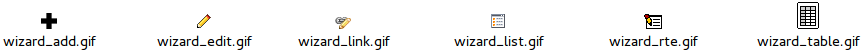
\includegraphics[width=0.95\linewidth]{DeprecatedRemovedFunctions/77630.png}
	\end{figure}

\end{frame}

% ------------------------------------------------------------------------------
% LTXE-SLIDE-START
% LTXE-SLIDE-UID:		e0eabd14-ba6cd6f1-10eb9443-dcad6904
% LTXE-SLIDE-ORIGIN:	d5ced5e7-04dffe16-b8ec9f2c-712020cd English
% LTXE-SLIDE-TITLE:		#77693: Remove/Move Icons from EXT:t3skin
% ------------------------------------------------------------------------------

\begin{frame}[fragile]
	\frametitle{Verouderde/verwijderde functies}
	\framesubtitle{Iconen uit \texttt{EXT:t3skin}}

	\begin{itemize}

		\item Iconen uit \texttt{EXT:t3skin} zijn verwijderd of verplaatst
		\item \textbf{Verwijderd:}

			\begin{itemize}
				\item \smaller\texttt{typo3/sysext/t3skin/icons/gfx/error.png}
				\item \texttt{typo3/sysext/t3skin/icons/gfx/i/\_icon\_ftp.gif}
				\item \texttt{typo3/sysext/t3skin/icons/gfx/information.png}
				\item \texttt{typo3/sysext/t3skin/icons/gfx/notice.png}
				\item \texttt{typo3/sysext/t3skin/icons/gfx/warning.png}
			\end{itemize}

		\item \textbf{Verplaatst:}

			\begin{itemize}
				\item \smaller\texttt{typo3/sysext/t3skin/icons/gfx/icon\_fatalerror.gif}
				\item \texttt{typo3/sysext/t3skin/images/icons/status/status-edit-read-only.png}
				\item \texttt{typo3/sysext/t3skin/images/icons/status/warning-in-use.png}
				\item \texttt{typo3/sysext/t3skin/images/icons/status/warning-lock.png}
				\item \texttt{typo3/sysext/t3skin/images/icons/status/status-reference-hard.png}
				\item \texttt{typo3/sysext/t3skin/images/icons/status/status-reference-soft.png}
			\end{itemize}

	\end{itemize}

\end{frame}

% ------------------------------------------------------------------------------
% LTXE-SLIDE-START
% LTXE-SLIDE-UID:		9b19852b-ad65c6fc-03eb87c9-ec43e516
% LTXE-SLIDE-ORIGIN:	7848f0b0-d687b337-f7638646-680dc819 English
% LTXE-SLIDE-TITLE:		Obsolete page tree and click menu settings removed
% ------------------------------------------------------------------------------

\begin{frame}[fragile]
	\frametitle{Verouderde/verwijderde functies}
	\framesubtitle{Paginaboom- en klikmenu-instellingen}

	\begin{itemize}

		\item Verouderde paginaboom- en klikmenu-instellingen zijn verwijderd
		\item \textbf{Eigenschappen}:

		\begin{itemize}
			\item \texttt{FileSystemNavigationFrameController->doHighlight}
			\item \texttt{ClickMenu->leftIcons}
		\end{itemize}

		\item \textbf{TypoScript-instellingen}:

		\begin{itemize}
			\item \texttt{options.pageTree.disableTitleHighlight}
			\item \texttt{options.contextMenu.options.leftIcons}
		\end{itemize}

	\end{itemize}

\end{frame}

% ------------------------------------------------------------------------------
% LTXE-SLIDE-START
% LTXE-SLIDE-UID:		39d5f363-921e3b35-9f9dd8a2-7a76f8d3
% LTXE-SLIDE-ORIGIN:	aad23a73-7b046eaf-fb4bb862-2f88ef71 English
% LTXE-SLIDE-TITLE:		ExtensionManagementUtility::extRelPath()
% LTXE-SLIDE-REFERENCE:	#78193: ExtensionManagementUtility::extRelPath() deprecated
% ------------------------------------------------------------------------------

\begin{frame}[fragile]
	\frametitle{Verouderde/verwijderde functies}
	\framesubtitle{ExtensionManagementUtility::extRelPath()}

	\begin{itemize}

		\item De methode \texttt{ExtensionManagementUtility::extRelPath()} is aangemerkt als verouderd
		\item Deze methode werd gebruikt voor het bepalen van relatieve paden
		\item Er zijn alternatieve methoden beschikbaar:

			\begin{itemize}
				\item \texttt{ExtensionManagementUtility::extPath()}\newline
					(voor het volledige pad van een extensie)
				\item \texttt{ExtensionManagementUtility::siteRelPath()}\newline
					(voor de relatieve locatie van de extensie t.o.v. \texttt{PATH\_site})
				\item \texttt{GeneralUtility::getFileAbsFileName()}\newline
					(voor bestandspaden die zijn voorgevoegd met EXT:myextension)
				\item \texttt{PathUtility::getAbsoluteWebPath()}\newline
					(voor locaties met een absolute verwijzing naar een webfolder)
			\end{itemize}

	\end{itemize}

\end{frame}

% ------------------------------------------------------------------------------
% LTXE-SLIDE-START
% LTXE-SLIDE-UID:		60f5c5c9-52d7c347-548bc02b-17085f7b
% LTXE-SLIDE-ORIGIN:	43a5eaf5-8945a8d5-ac27d4ea-24ffc8e3 English
% LTXE-SLIDE-TITLE:		Miscellaneous (1) (#75363)
% LTXE-SLIDE-REFERENCE:	#75363: Deprecate FormResultCompiler->JStop()
% LTXE-SLIDE-REFERENCE:	#75637: Deprecate optional parameters of RecyclerUtility::getRecordPath()
% ------------------------------------------------------------------------------

\begin{frame}[fragile]
	\frametitle{Verouderde/verwijderde functies}
	\framesubtitle{Divers (1)}

	\begin{itemize}
		\item Methode \texttt{FormResultCompiler->JStop()} is hernoemd naar \texttt{addCssFiles()}.
			De oude methodenaam blijft aanwezig als verouderde alias en zal in TYPO3 v9 worden verwijderd.

		\item Methode \texttt{ClickMenu::DB\_editPageProperties()} is aangemerkt als verouderd

		\item De volgende argumenten van methode \texttt{RecyclerUtility::getRecordPath()} zijn aangemerkt als verouderd:
			\begin{itemize}
				\item \texttt{\$clause}
				\item \texttt{\$titleLimit}
				\item \texttt{\$fullTitleLimit}
			\end{itemize}

	\end{itemize}

\end{frame}

% ------------------------------------------------------------------------------
% LTXE-SLIDE-START
% LTXE-SLIDE-UID:		6fdd648b-e3e958d7-9c122b3b-23478ebb
% LTXE-SLIDE-ORIGIN:	0745e3f3-83db03d7-ac24e92a-300391ba English
% LTXE-SLIDE-TITLE:		Miscellaneous (2) (#77783 and #77826)
% LTXE-SLIDE-REFERENCE:	#77783: Unused ExtJS JavaScript libraries removed
% LTXE-SLIDE-REFERENCE:	#77826: RTEHtmlArea Spellchecker eID removed
% ------------------------------------------------------------------------------

\begin{frame}[fragile]
	\frametitle{Verouderde/verwijderde functies}
	\framesubtitle{Divers (2)}

	\begin{itemize}

		\item De volgende ongebruikte ExtJS-bibliotheken zijn verwijderd:

			\begin{itemize}
				\item \texttt{app.SearchField}
				\item \texttt{grid.RowExpander}
				\item \texttt{ux.FitToParent}
			\end{itemize}

		\item De RTEHtmlArea eID (\texttt{rtehtmlarea\_spellchecker}) voor het gebruik van 
			dynamische spellingcontroles is verwijderd en het entry point voor HTTP-requests
			\texttt{SpellCheckingController->main} is aangemerkt als verouderd

		\item \texttt{DateTime::ISO8601} is incompatible met ISO-8601,
			maar is nog aanwezig voor achterwaartse compatibiliteit. In plaats daarvan worden
			de constanten \texttt{DateTime::ATOM} of \texttt{DATE\_ATOM} gebruikt.

	\end{itemize}

\end{frame}

% ------------------------------------------------------------------------------
% LTXE-SLIDE-START
% LTXE-SLIDE-UID:		0cc7b010-62ccdd5b-b8580a4c-3af78138
% LTXE-SLIDE-ORIGIN:	0745e3f3-83db03d7-ac24e92a-300391ba English
% LTXE-SLIDE-TITLE:		Miscellaneous (3) (#77839, #78096 and #78222)
% LTXE-SLIDE-REFERENCE:	#77839: TYPO3/CMS/Core/QueryGenerator
% LTXE-SLIDE-REFERENCE:	#78096: Deprecate PageLayoutView::getResult with mysqli_result objects
% LTXE-SLIDE-REFERENCE:	#78222: Late generation of autoload information is deprecated
% ------------------------------------------------------------------------------

\begin{frame}[fragile]
	\frametitle{Verouderde/verwijderde functies}
	\framesubtitle{Divers (3)}

	\begin{itemize}

		\item De AMD-module \texttt{TYPO3/CMS/Core/QueryGenerator} is verplaatst naar EXT:lowlevel\newline
			\small
				(en hernoemd naar \texttt{TYPO3/CMS/Lowlevel/QueryGenerator})
			\normalsize

		\item Methode \texttt{PageLayoutView::getResult()}, met \texttt{mysqli\_result}-objecten 
			als eerste parameter, is aangemerkt als verouderd

		\item Als TYPO3 zich in de non-Composer-modus bevond, werd de autoload-informatie relatief laat in het 
			bootstrapproces gedumpt. Dat gedrag is nu aangemerkt als verouderd.
	\end{itemize}

\end{frame}

% ------------------------------------------------------------------------------
